\section{Process' Perspective}

\subsection{Collaborative Development \& Team Organization}

At group formation, the team aligned expectations. Each member expected to spend 8-12 hours a week on the course, resulting in this schedule:

\begin{itemize}
    \item Tuesday, 10-14: Project Work
    \item Tuesday, 14-16: Lecture
    \item Tuesday, 16-18: Exercises/Project Work
    \item Friday, 10-15: Project Work
\end{itemize}

All sessions were in person. Each member had the freedom to do additional work. Communication was through Discord \autocite{discord}.

When working, we would at times do versions of pair programming. Teamwork was however difficult, since all concepts were new to everybody, and a lot of the understanding and progress came from trial and error. All sessions were an open forum where questions were welcome, and help was always possible to get. Sadly, we were not always good at remembering co-authorship on commits which might make the repository contributions look skewed.

We intended to utilize GitHub Issues to share the tasks between us, making sure not to be wasting time on duplicate work \autocite{github-issues}.

\subsection{CI/CD Chain}
In this project, we have implemented a CI/CD chain by defining a handful of \texttt{.yml} files for GitHub Actions. A visual representation can be seen at figure \ref{fig:CI/CD Overview}: 

\begin{itemize}
    \item github-super-linter
    \item dotnet-Build-and-Test
    \item container-snyk
    \item continuous-deployment
    \item dotnet-format
    \item Scheduled-release
    \item latex-build
\end{itemize}

We also configured Dependabot, that scans for outdated dependencies and informs us of updates through pull requests \autocite{dependabot}.

Dotnet-build-and-Test, container-snyk and dotnet-format run simultaneously every time a pull request is created. As part of our workflow, no pull requests were supposed to be merged into main without having a developer review it first. This was not entirely adhered to, however.

Every push to feature branches triggered the Super-linter. The first thing that happens when a pull request is created is that the application is built. We only build the application after pull requests, to avoid running unnecessary build cycles, reducing overhead. The dotnet-format workflow then operates on the build to guarantee a greater level of code consistency. Our build workflow then proceeds by checking out the branch, restoring the dependencies, building the application and executing the unit tests. This makes the test-stage dependant on the build-stage; if the build fails, the tests are never run. Depending on the test-suite, stability is ensured by making sure changes are tested, and old functionalities do not break (regression testing) \autocite{regression-testing}.

The Snyk workflow does security scans on the repository and notifies us of any vulnerabilities in open-source dependencies. Additionally, to mitigate the risk of inadvertently exposing secrets, we used a Snyk feature on our code base to scan for sensitive data like connection strings, secret tokens, API keys, etc.

If either the building or testing fails, the pull request will be rejected.

\begin{figure}
    \centering
    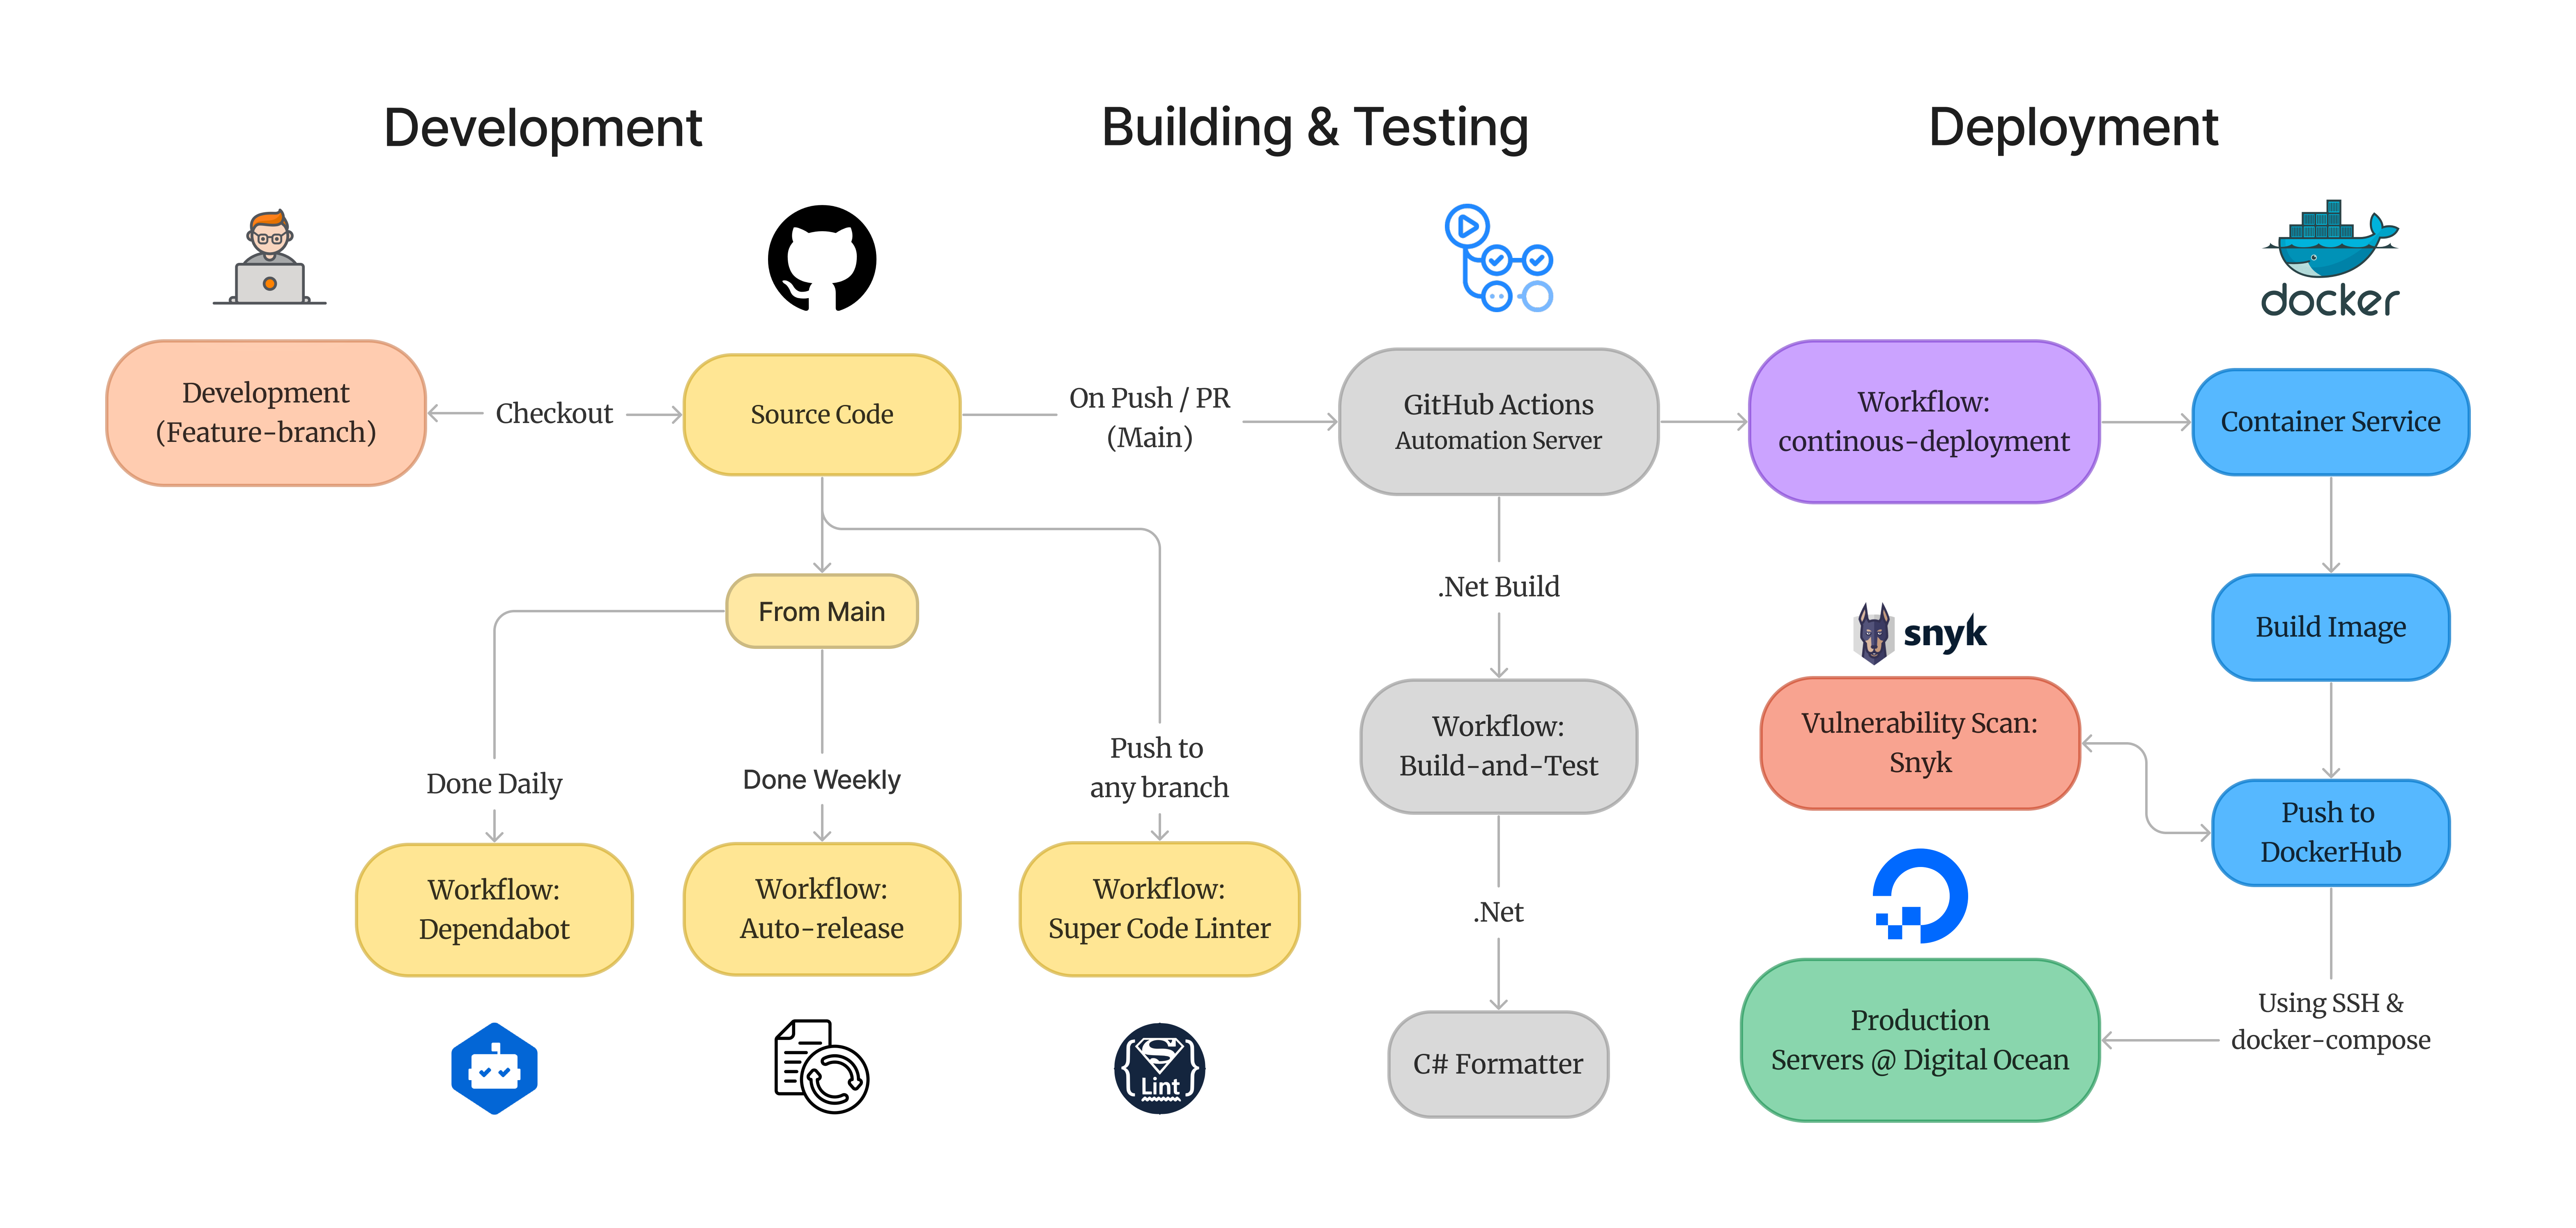
\includegraphics[width=1.0\linewidth]{Images/CICD_Chain.png}
    \caption{CI/CD tech-stack}
    \label{fig:CI/CD Overview}
\end{figure}

% Deployment workflow in detail:
The continous-deployment workflow has the purpose of automatically deploying our services. It builds the containers and connects to the cloud droplets and deploys.

Combined with the use of GitHub Secrets, these workflows provide a powerful solution to automated deployment \autocite{github-secrets}. It's a convenient way to manage our application's deployment process, while maintaining confidentiality and flexibility. This solution does however make scalability difficult because of hardcoded IP-addresses of our servers. This makes any changes tedious, as they would require manual changes to workflows and secrets.

The latex-build workflow only runs when files changed include those in the Report folder. It compiles the components of the report to a .pdf.

% (Release) workflow
The auto-release workflow was implemented to further streamline the deployment process. It ensures that the latest changes are automatically released, scheduled for each Sunday at 20:00 CEST. 

\subsection{Repository Organization \& Development Strategy}
\subsubsection{Repository Organization}

We structured our code in a mono-repository for two main reasons:
\begin{enumerate}
    \item It provides improved collaboration, as all developers are working on the same codebase.
    \item It simplifies version control as we only have a single history for all code.
\end{enumerate}
Another consideration was, that we didn't feel the need to divide it up, as the application is still relatively small. It would also add what we deemed to be unnecessary complexity by requiring different repositories to be cloud-hosted for cross-access since the necessary references in our C\# code would no longer reside in the same .NET solution.


\subsubsection{Development Strategy}
We utilized feature branching which adds security gates from a require-to-pass test suite run in GitHub Actions and code reviews from other devs \autocite{github-actions}. Main was intended to be secured by only allowing pushes through pull requests, but we allowed direct pushes as setting up secrets and editing workflows proved time-consuming otherwise.

Our tasks were organized in GitHub Issues. This made it possible for each member to always be able to see which tasks were up for grabs, and who were working on what. It also acted as a task backlog giving an overview of the work that was yet to be done.

As the project progressed, however, the tasks began including the whole group, and the Issues board became slightly irrelevant.

\subsection{Monitoring \& Logging}
%How do you monitor your systems and what precisely do %you monitor?
%What do you log in your systems and how do you %aggregate logs?

\subsubsection{Monitoring} \label{Monitoring}
The monitoring of the system is powered by Prometheus which gathers metrics from endpoints created by the Prometheus.net NuGet package \autocite{prometheus}. Metrics are then visualized by Grafana which queries Prometheus \autocite{grafana}. Though Grafana is available to anyone, you would need our login to access the metrics and dashboards. Our current metrics are:

\begin{itemize}
    \item Http-requests (Duration)
    \item Total Users
    \item Total Messages
    \item Average request duration (Last 2 minutes)
\end{itemize}

\noindent Together, these metrics provide information about how much stress we can expect our system to experience, and what kind of request intensity we can expect. It also provides an overview of user growth, giving us a sense of the direction our service is headed. 

Additionally, we are also making use of Digital Ocean to monitor our hardware such as the CPU and memory usage of our droplets.

\subsubsection{Logging} \label{Logging}

Our projects logging is accomplished using the Serilog library, which is a popular logger for C\# \autocite{serilog}. We send the logs to ElasticSearch which stores and indexes them, allowing for fast and efficient lookups \autocite{elasticsearch}. We use Kibana as a UI to view the log files \autocite{kibana}.

Serilog provides the ability to have multiple sinks, which are output destinations. We have a sink to ElasticSearch and the console of the container. 

%Maybe deletings:
To tie Serilog and ElasticSearch together with Kibana, we made a docker-compose file responsible for setting up the connection and mounting the data from the container. Kibana then retrieves the logging data from ElasticSearch and displays it.
% to herings ^
\subsection{Security Assessment}

Our security assessment consisted of a penetration test - Zed Attack Proxy, or ZAP, that showed some flaws in our program \autocite{zap}. Most seemed to be relatively simple to fix, and none seemed to be too severe in nature:
\begin{itemize}
    \item No Anti-CSRF tokens were found in an HTML submission form
    \item Passive (90022 - Application Error Disclosure)
    \item Content Security Policy (CSP) Header Not Set
    \item Missing Anti-clickjacking Header
    \item X-Content-Type-Options Header Missing
    \item Hidden File Found
    \item Vulnerable JS Library
    \item XSLT Injection might be possible.
    \item Cloud Metadata Potentially Exposed
\end{itemize}

\noindent These items resulted in GitHub Issues; some of which were dealt with while others were down-prioritized.

\subsection{Scaling \& Load Balancing}
%Applied strategy for scaling and load balancing. 

Our applied strategy for scaling and load balancing involved utilizing Docker Swarm for fault tolerance and easy container management, together with Nginx working primarily as a load balancer and reverse proxy \autocite{docker-swarm, nginx}. Docker Swarm uses a cluster of nodes (workers and managers) and allows us to automatically adjust the number of running Docker containers based on the current workload. Another important feature of the swarm is that it automatically evenly distributes incoming requests, across the worker containers running the same service (internal load balancing with an ingress mesh).

The swarm has a maximum capacity limited to the combined resources (CPU, memory, disk space) of the server nodes within the swarm clusters. We used two servers for our application swarm and one server for the load-balancing swarm.

The first swarm consists of a server with manager nodes and a server with worker nodes running containers with our MiniTwit application. The second swarm includes a single manager node responsible for load balancing and reverse-proxying with Nginx. We designed it this way to separate concerns and allow the two swarms to scale independently. Combining Docker Swarm's automatic and dynamic scaling with Nginx's reverse-proxy capabilities resulted in an improvement in the system's availability and reliability.

By having Nginx handle and redirect requests to our service, we could eliminate the 'single point of failure', and decrease the impact a server crash has on our system. In case the primary replica node running our swarm was flooded or broke down, we could redirect the traffic from that server node to another upstream server, while docker swarms dynamical scaling would ensure that the system would be able to keep up with accelerating requests and users.

However, in our setup, there were a couple of things that could be improved.
Initially, we only tested our system using a single instance of Nginx, which essentially only shifted the single point of failure from the application service to the load balancer in the Swarm. This decision involved weighing the trade-offs between reliability, complexity, and also the financial costs of creating more droplets.
Also, we encountered some non-negligible internal network delays that affected the system's performance. When Nginx was responsible for the load balancing, requests sometimes took a long time to complete or re-direct. Due to the way Nginx was implemented, it didn't function as originally intended.


\subsection{AI Assistance}

As developers, we have embraced the tool that is AI. We have used ChatGPT as a sparring partner whenever we got a task we did not know how to solve, or when we got stuck \autocite{chatgpt}. It has mostly been good at providing ideas or starting points. But where it really shines is when troubleshooting or debugging. If nothing else, it has provided the services of a rubber duck \autocite{rubber-duck-debugging}.

We have also used it in the formulation of documents like the SLA agreement, as it's mostly boilerplate text anyways. We provided it with some information about our system and what guarantees we could give, and it returned a rough draft we could finalize.

Finally, one team member has been using GitHub Copilot \autocite{github-copilot} as an advanced intellisense tool, but not for making several lines of code. Meaning that it was used to finish individual lines of code, but not for making entire methods or blocks of code.